\vspace{-1.5cm}
\begin{IEEEbiography}[{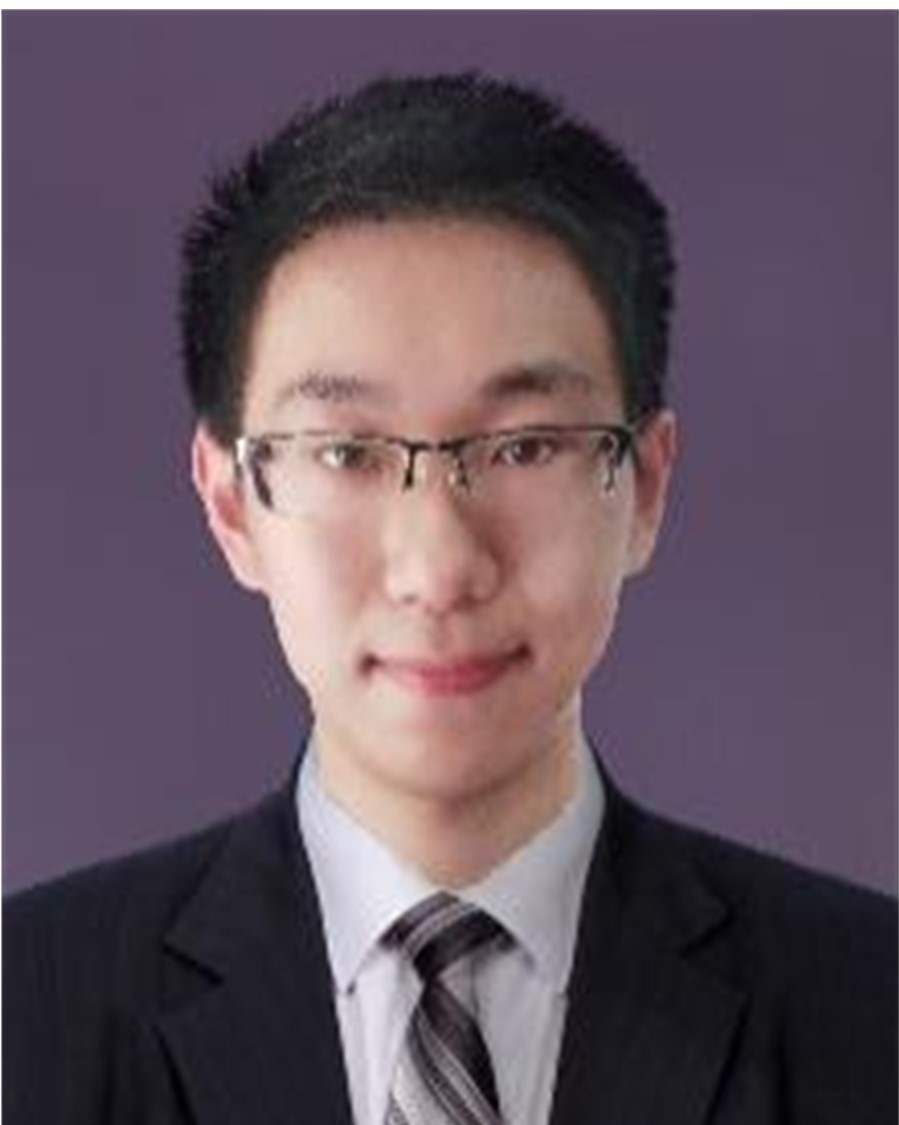
\includegraphics[width=1in,height=1.25in,clip,keepaspectratio]{fig/XiaojingQI.jpg}}]{Xiaojing Qi}
was born in 2000. He received his B.S. degree from Jilin University, Jilin, China, in 2023. He is pursuing his master’s degree in vehicle engineering at the School of Vehicle and Mobility, Tsinghua University, Beijing, China. His research interests include automotive computational fluid dynamics, and vehicle simulation and control, especially regarding the rollover stability control of tank trucks under cloud control systems, cloud-based predictive lane change control, cloud-based predictive cruise control, and cloud control architecture.

E-mail: qxj23@mails.tsinghua.edu.cn
\end{IEEEbiography}
\vspace{-1.2cm}

\begin{IEEEbiography}[{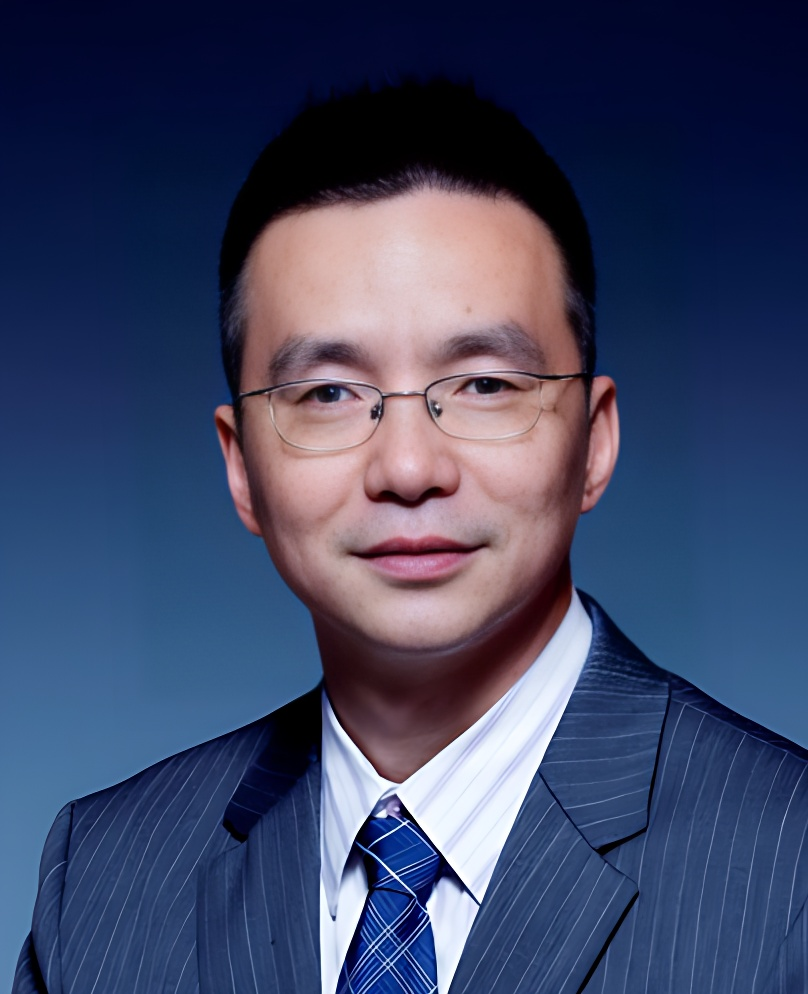
\includegraphics[width=1in,height=1.25in,clip,keepaspectratio]{fig/YugongLUO.png}}]{Yugong Luo}
received the B.S. and M.S. degrees in mechanical engineering from Chongqing University, Chongqing, China, and the Ph.D. degree in mechanical engineering from Tsinghua University, Beijing, China, in 1996, 1999, and 2003, respectively.

He is currently a Professor with the School of Vehicle and Mobility, Tsinghua University. He was a Visiting Scientist with the Department of Mechanical Engineering, University of Michigan Ann Arbor, MI, USA, in 2013 and 2014. He is a coauthor of four books. His research interests include intelligent vehicles, hybrid electric vehicles, and multiobjective control.

E-mail: lyg@tsinghua.edu.cn 
\vspace{-1.2cm}
\end{IEEEbiography}


\begin{IEEEbiography}[{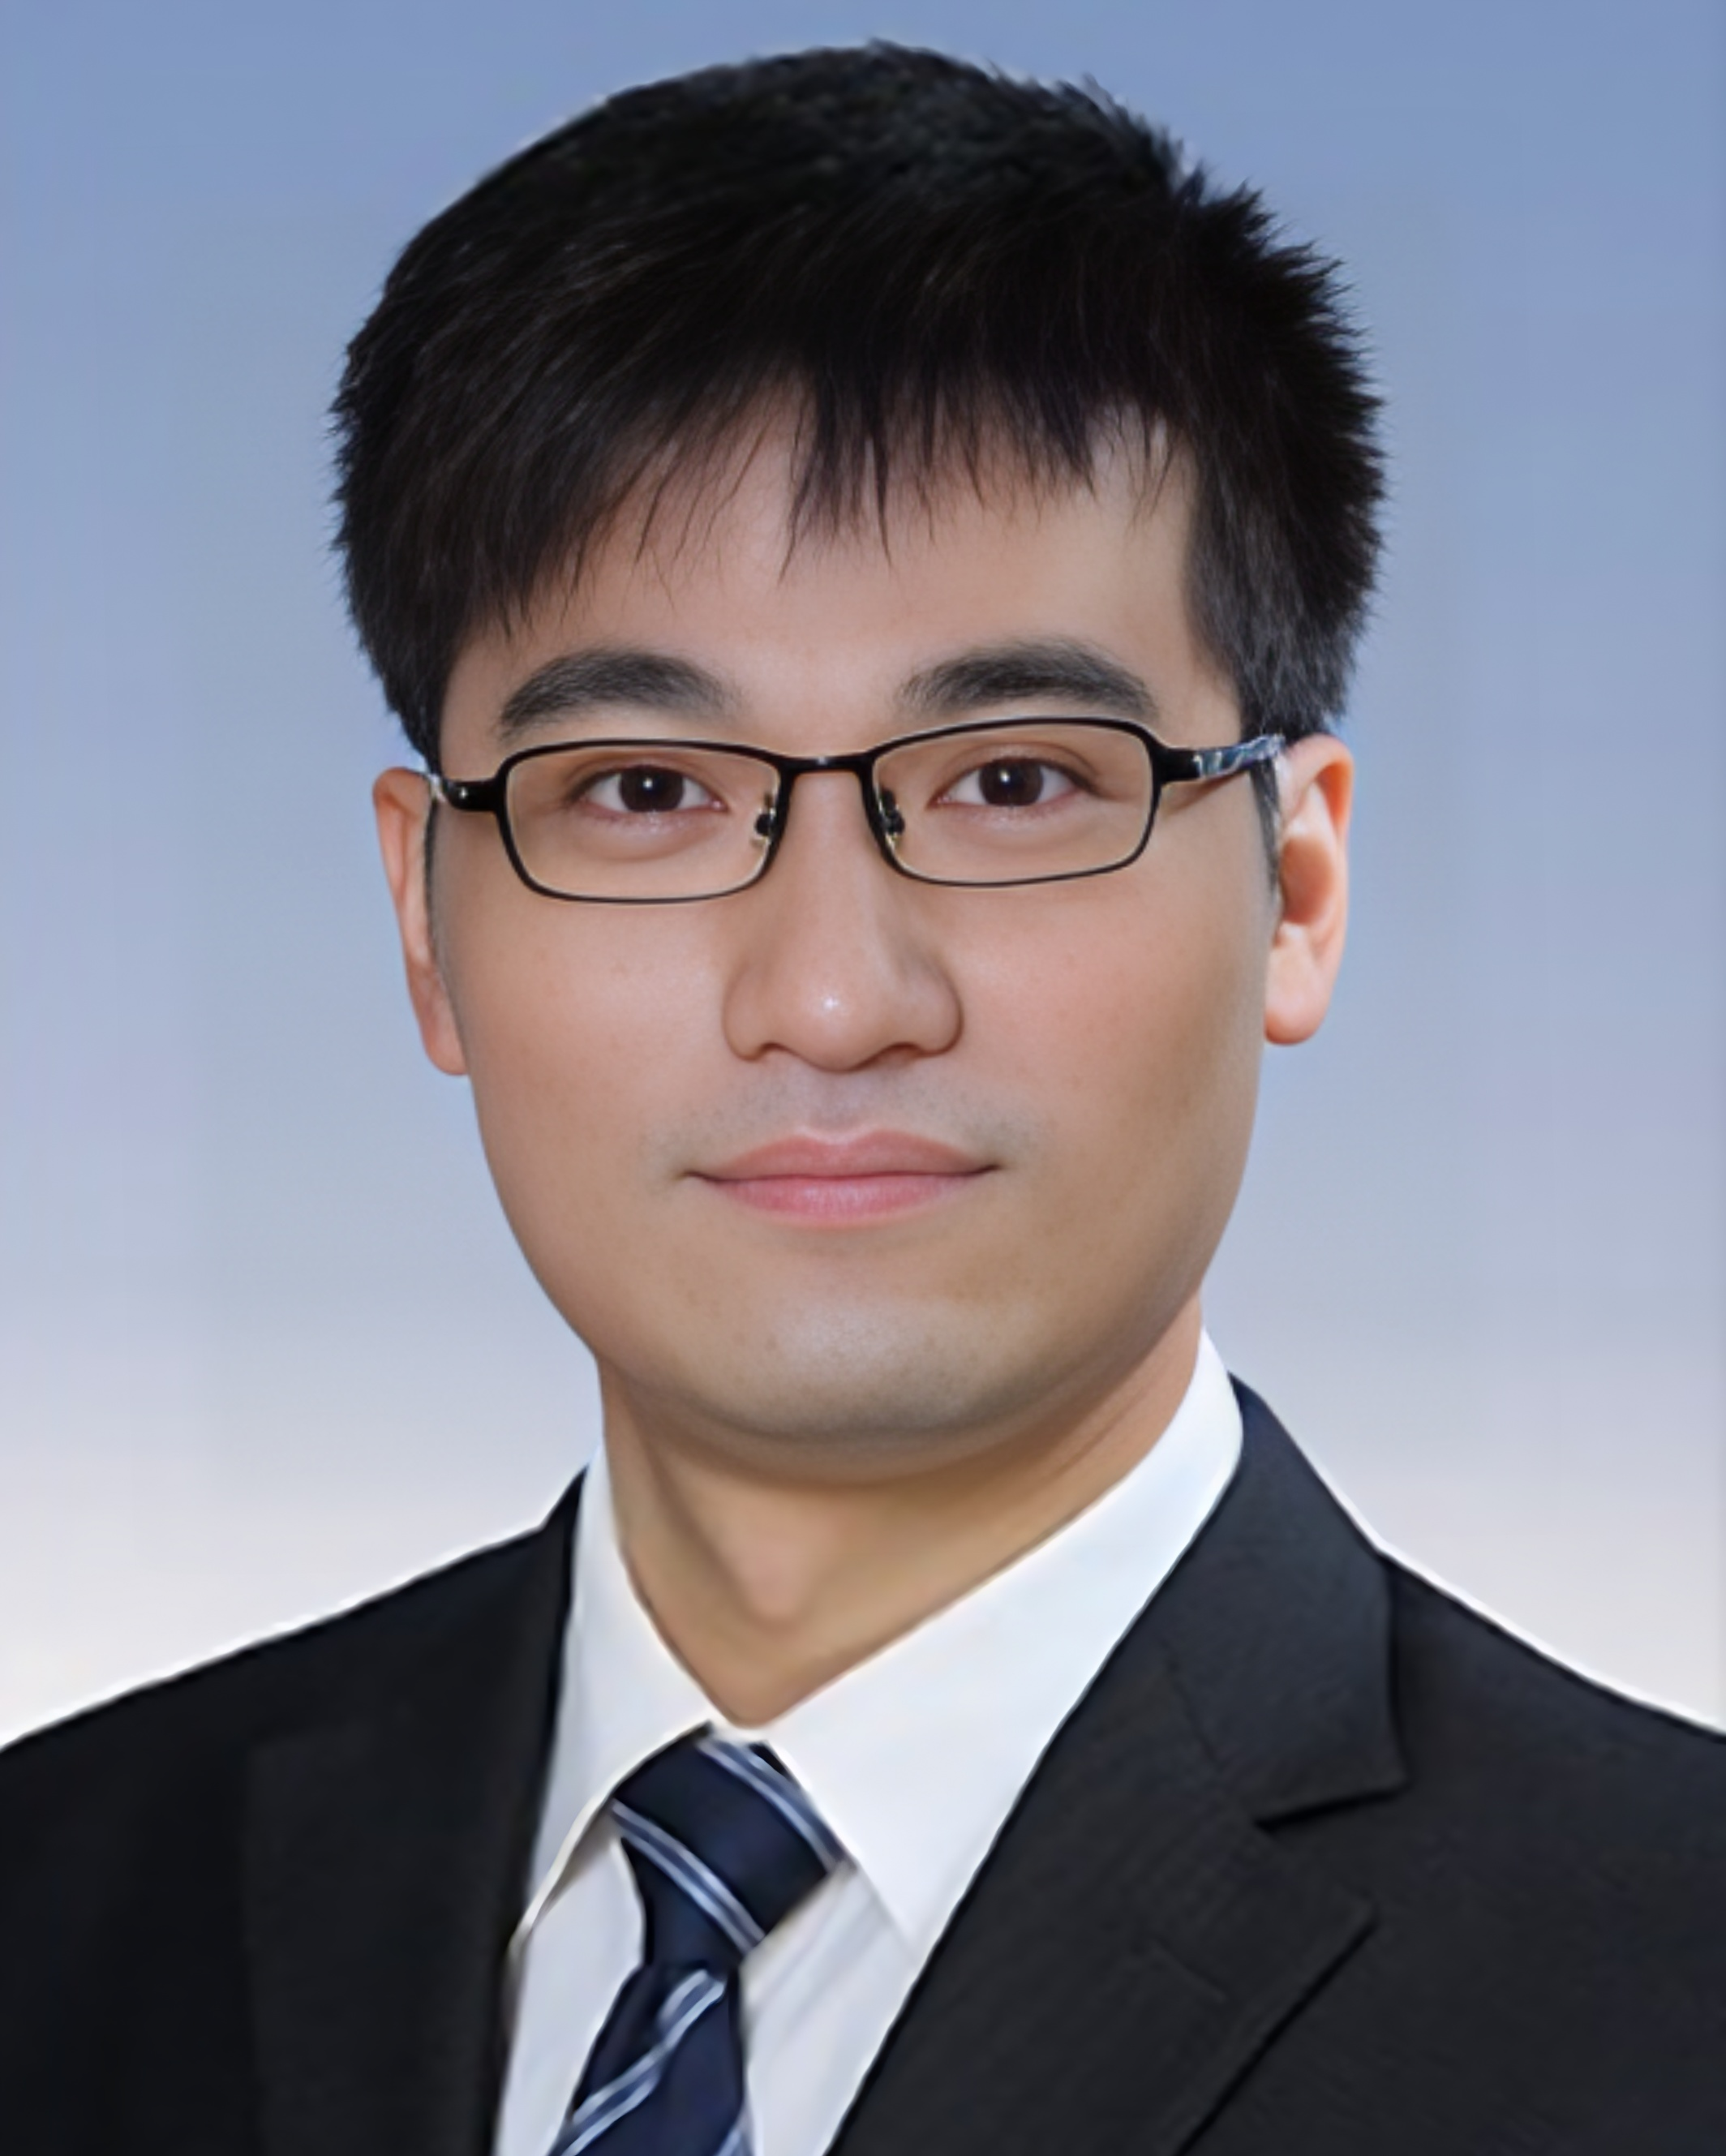
\includegraphics[width=1in,height=1.25in,clip,keepaspectratio]{fig/BolinGAO.jpg}}]{Bolin Gao}
was born in 1986. He is now an associate research professor at the School of Vehicle and Mobility, Tsinghua University. His research interests include the theoretical research and engineering application of the dynamic design and control of intelligent and connected vehicles, especially about the collaborative perception and tracking method in cloud control systems, intelligent predictive cruise control systems on commercial trucks with cloud control mode, as well as the test and evaluation of intelligent vehicle driving systems.

E-mail: gaobolin@tsinghua.edu.cn
\vspace{-1.2cm}
\end{IEEEbiography}

\begin{IEEEbiography}[{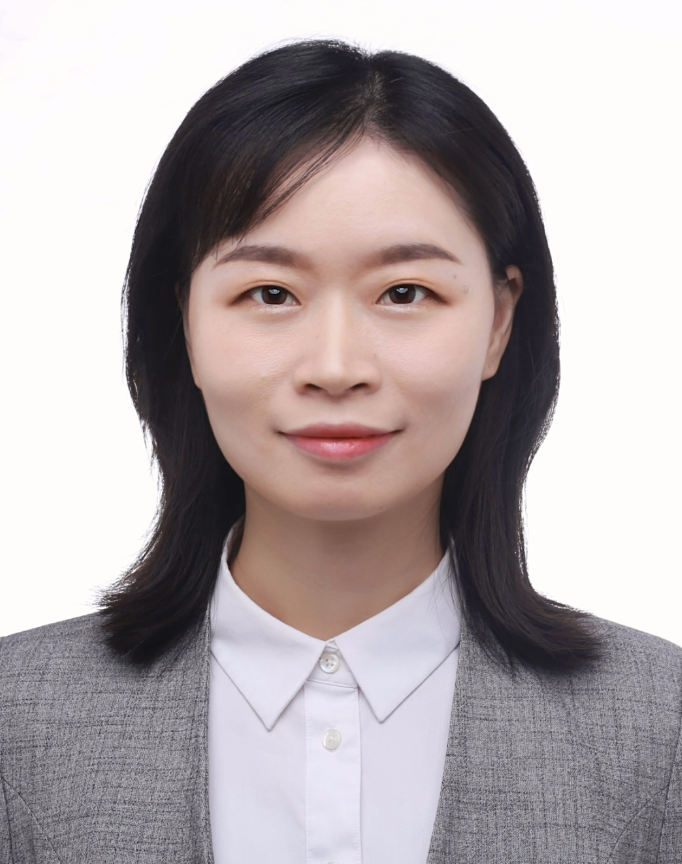
\includegraphics[width=1in,height=1.25in,clip,keepaspectratio]{fig/zhongwei.png}}]{Wei Zhong} received the B.S. and Ph.D. degrees in the School of Vehicle and Mobility, Tsinghua University, China, and used to be the chief at the National Innovation Center of Intelligent and Connected Vehicles, China. She is now an associate research professor at the School of Vehicle and Mobility, Tsinghua University. Her primary research focus is on the integrated design of vehicle-road-cloud integrated control systems, collaborative planning and control, systems engineering, and multi-objective optimization.

E-mail: zhongwei@mail.tsinghua.edu.cn
\end{IEEEbiography}
